%%
%% This is file `sample-manuscript.tex',
%% generated with the docstrip utility.
%%
%% The original source files were:
%%
%% samples.dtx  (with options: `manuscript')
%%
%% IMPORTANT NOTICE:
%%
%% For the copyright see the source file.
%%
%% Any modified versions of this file must be renamed
%% with new filenames distinct from sample-manuscript.tex.
%%
%% For distribution of the original source see the terms
%% for copying and modification in the file samples.dtx.
%%
%% This generated file may be distributed as long as the
%% original source files, as listed above, are part of the
%% same distribution. (The sources need not necessarily be
%% in the same archive or directory.)
%%
%% Commands for TeXCount
%TC:macro \cite [option:text,text]
%TC:macro \citep [option:text,text]
%TC:macro \citet [option:text,text]
%TC:envir table 0 1
%TC:envir table* 0 1
%TC:envir tabular [ignore] word
%TC:envir displaymath 0 word
%TC:envir math 0 word
%TC:envir comment 0 0
%%
%%
%% The first command in your LaTeX source must be the \documentclass command. This is the generic manuscript mode required for submission and peer review.
% \documentclass[acmsmall,screen,review,anonymous]{acmart}
\documentclass[acmsmall,screen,review]{acmart}

\usepackage{xspace}
\usepackage{listings}
\newcommand{\todo}[1]{{\color{red} #1}}

%% To ensure 100% compatibility, please check the white list of
%% approved LaTeX packages to be used with the Master Article Template at
%% https://www.acm.org/publications/taps/whitelist-of-latex-packages
%% before creating your document. The white list page provides
%% information on how to submit additional LaTeX packages for
%% review and adoption.
%% Fonts used in the template cannot be substituted; margin
%% adjustments are not allowed.

%%
%% \BibTeX command to typeset BibTeX logo in the docs
\AtBeginDocument{%
  \providecommand\BibTeX{{%
    \normalfont B\kern-0.5em{\scshape i\kern-0.25em b}\kern-0.8em\TeX}}}

%% Rights management information.  This information is sent to you
%% when you complete the rights form.  These commands have SAMPLE
%% values in them; it is your responsibility as an author to replace
%% the commands and values with those provided to you when you
%% complete the rights form.
\setcopyright{acmcopyright}
\copyrightyear{2018}
\acmYear{2018}
\acmDOI{XXXXXXX.XXXXXXX}

%% These commands are for a PROCEEDINGS abstract or paper.
% \acmConference[Conference acronym 'XX]{Make sure to enter the correct
%   conference title from your rights confirmation emai}{June 03--05,
%   2018}{Woodstock, NY}
%
%  Uncomment \acmBooktitle if th title of the proceedings is different
%  from ``Proceedings of ...''!
%
%\acmBooktitle{Woodstock '18: ACM Symposium on Neural Gaze Detection,
%  June 03--05, 2018, Woodstock, NY}

%% These commands are for a JOURNAL article.
\acmJournal{JACM}
\acmVolume{37}
\acmNumber{4}
\acmArticle{111}
\acmMonth{8}

\acmPrice{15.00}
\acmISBN{978-1-4503-XXXX-X/18/06}


%%
%% Submission ID.
%% Use this when submitting an article to a sponsored event. You'll
%% receive a unique submission ID from the organizers
%% of the event, and this ID should be used as the parameter to this command.
%%\acmSubmissionID{123-A56-BU3}

%%
%% For managing citations, it is recommended to use bibliography
%% files in BibTeX format.
%%
%% You can then either use BibTeX with the ACM-Reference-Format style,
%% or BibLaTeX with the acmnumeric or acmauthoryear sytles, that include
%% support for advanced citation of software artefact from the
%% biblatex-software package, also separately available on CTAN.
%%
%% Look at the sample-*-biblatex.tex files for templates showcasing
%% the biblatex styles.
%%

%%
%% The majority of ACM publications use numbered citations and
%% references.  The command \citestyle{authoryear} switches to the
%% "author year" style.
%%
%% If you are preparing content for an event
%% sponsored by ACM SIGGRAPH, you must use the "author year" style of
%% citations and references.
%% Uncommenting
%% the next command will enable that style.
%%\citestyle{acmauthoryear}

%%
%% end of the preamble, start of the body of the document source.
\begin{document}

%%
%% The "title" command has an optional parameter,
%% allowing the author to define a "short title" to be used in page headers.
\title{Semi-Automated Direction-Driven Functional Conversion}
%%
%% The "author" command and its associated commands are used to define
%% the authors and their affiliations.
%% Of note is the shared affiliation of the first two authors, and the
%% "authornote" and "authornotemark" commands
%% used to denote shared contribution to the research.
\author{Ekaterina Verbitskaia}
\email{kajigor@gmail.com}
% \orcid{\todo{1234-5678-9012}}
\affiliation{%
  \institution{JetBrains Research}
  \city{Belgrade}
  \country{Serbia}
}

\author{Igor Engel}
\email{abc@def.com}
% \orcid{\todo{1234-5678-9012}}
\affiliation{%
  \institution{JetBrains Research}
  \city{Bremen}
  \country{Germany}
}

\author{Daniil Berezun}
\email{abc@def.com}
% \orcid{\todo{1234-5678-9012}}
\affiliation{%
  \institution{JetBrains Research}
  \city{Amsterdam}
  \country{Netherlands}
}


%%
%% By default, the full list of authors will be used in the page
%% headers. Often, this list is too long, and will overlap
%% other information printed in the page headers. This command allows
%% the author to define a more concise list
%% of authors' names for this purpose.
\renewcommand{\shortauthors}{Verbitskaia, Engel, Berezun}

%%
%% The abstract is a short summary of the work to be presented in the
%% article.
\begin{abstract}
 \todo{A clear and well-documented \LaTeX\ document is presented as an
  article formatted for publication by ACM in a conference proceedings
  or journal publication. Based on the ``acmart'' document class, this
  article presents and explains many of the common variations, as well
  as many of the formatting elements an author may use in the
  preparation of the documentation of their work.}
\end{abstract}

%%
%% The code below is generated by the tool at http://dl.acm.org/ccs.cfm.
%% Please copy and paste the code instead of the example below.
%%
\begin{CCSXML}
<ccs2012>
 <concept>
  <concept_id>10010520.10010553.10010562</concept_id>
  <concept_desc>Computer systems organization~Embedded systems</concept_desc>
  <concept_significance>500</concept_significance>
 </concept>
 <concept>
  <concept_id>10010520.10010575.10010755</concept_id>
  <concept_desc>Computer systems organization~Redundancy</concept_desc>
  <concept_significance>300</concept_significance>
 </concept>
 <concept>
  <concept_id>10010520.10010553.10010554</concept_id>
  <concept_desc>Computer systems organization~Robotics</concept_desc>
  <concept_significance>100</concept_significance>
 </concept>
 <concept>
  <concept_id>10003033.10003083.10003095</concept_id>
  <concept_desc>Networks~Network reliability</concept_desc>
  <concept_significance>100</concept_significance>
 </concept>
</ccs2012>
\end{CCSXML}

\ccsdesc[500]{Computer systems organization~Embedded systems}
\ccsdesc[300]{Computer systems organization~Redundancy}
\ccsdesc{Computer systems organization~Robotics}
\ccsdesc[100]{Networks~Network reliability}

%%
%% Keywords. The author(s) should pick words that accurately describe
%% the work being presented. Separate the keywords with commas.
\keywords{datasets, neural networks, gaze detection, text tagging}

\received{20 February 2007}
\received[revised]{12 March 2009}
\received[accepted]{5 June 2009}

%%
%% This command processes the author and affiliation and title
%% information and builds the first part of the formatted document.
\maketitle



\section{Introduction}

Implementing a program is often significantly easier than its inversion.
For example, integer multiplication is much simpler than factoring, while program evaluation is easier than program generation.
Although inversion is undecidable, there are approaches capable of inversing a computation in some cases, notably, universal resolving algorithm \todo{cite Gluck}, logic and relational programming.
Inversion comes with a lot of overhead which may be reduced in some circumstances.
% The focus of this paper is to reduce overhead when implementing inversions of  programs written in \mk by translating them into functional counterparts.

One source of overhead in relational programming comes from \emph{unification} --- the basic operation which is at the core of \mk.
Unification involves traversing terms being unified along with a list of substitutions and doing occurs-check all of which may be redundant when there is a specific execution \emph{direction} in mind.
Directions fix at compile-time which arguments of a relation are always going to be known and ground at runtime.
Having this information, it is possible to specialize a relation for the direction \todo{cite Verbitskaia} and get rid of some of the overhead.
In this case, unifications may prove to be redundant and be replaced with much simpler pattern-matching and equality checks.

In this paper we present a scheme of translation of \mk programs into a host functional programming language as a sequence of examples.
Examples start from the simplest translations and evolve to introduce different features of \mk which influence translation.
Currently translation is not automated: everything is done manually.
We believe the translation can be semi-automated, leaving some decisions up to a programmer.
Although this project is at the early state, evaluation demonstrates its usefulness by significantly speeding up such programs as computing a topological sorting of a graph and generating logic formulas which evaluate to the given value.


\section{Background}

In this section, we give the abstract syntax of \micro version used in this paper and describe a concept of modes which was developed earlier for other logic languages.

\subsection{Normal Form Abstract Syntax of \micro}

To simplify the functional conversion scheme, we consider \micro relations to be in the superhomogeneous normal form used in the \merc programming language~\cite{somogyi1996execution}.
Converting an arbitrary \micro relation into the normal form is a simple syntactic transformation, which we omit.

In the normal form, a term is either a variable or a constructor application which is flat and linear.
Linearity means that arguments of a constructor are distinct variables.
To be flat, a term should not contain any nested constructors.
Each constructor has a fixed arity $n$.
Below is the abstract syntax of the term language over the set of variables $V$.
\[  \FlatTerm_{V} = V \cup \{\Cons_{n}\left( x_1, \ldots, x_{n} \right) \mid x_{i}\in V; i \neq j \Rightarrow x_i \neq x_j\} \]

Whenever a term which does not adhere to this form is encountered in a unification or as an argument of a call, it is transformed into a conjunction of several unifications, as illustrated by the following examples:
\begin{equation*}
\begin{split}
C\left( x_1, x_2 \right) \equiv C\left( C\left( y_1, y_2 \right), y_3 \right) & \Rightarrow x_1 \equiv C\left( y_1, y_2 \right) \land x_2 \equiv y_3 \\
C\left( C\left( x_1, x_2 \right), x_3 \right) \equiv C\left( C\left( y_1, y_2 \right), y_3 \right) & \Rightarrow  x_1 \equiv y_1 \land x_2 \equiv y_2 \land x_3 \equiv y_3 \\
x \equiv C \left(y, y \right) & \Rightarrow x \equiv C \left(y_1, y_2\right) \land y_1 \equiv y_2 \\
add^o\left( x, x, z \right) & \Rightarrow add^o\left( x_1, x_2, z \right) \land x_1 \equiv x_2
\end{split}
\end{equation*}

Unification in the normal form is restricted to always unify a variable with a term.
We also prohibit using disjunctions inside conjunctions.
The normalization procedure declares a new relation whenever this is encountered.

The complete abstract syntax of the \micro language used in this paper is presented in figure~\ref{fig:miniKanren}.

\begin{figure}[h]
    \begin{tabular}{llll}
     $\Def_{V}^N$ & $:$ & $R_{n}\left( x_1, \ldots, x_{n} \right) = \Disj_{V}, x_{i}\in V$ & normalized relation definition \\
    $\Disj_{V}$ & $:$ & $\bigvee\left( c_1, \ldots, c_{n} \right), c_{i}\in \Conj_{V}$ & normal form \\
    $\Conj_{V}$ & $:$ & $\bigwedge\left( g_1, \ldots, g_n \right), g_{i}\in \Base_{V}$ & normal conjunction \\
    $\Base_{V}$ & $:$ & $V \equiv \FlatTerm_{V}$ & flat unification \\
                & $\mid$ & $R_{n}\left( x_1, \ldots, x_{n} \right), x_{i}\in V, i \neq j \Rightarrow x_i \neq x_j$ & flat call\\

    % $\Delay$ & $:$ &  $\text{Delay} \mid \text{NoDelay} $ &
    \end{tabular}
    \caption{Abstract syntax of \micro in the normal form}
    \label{fig:miniKanren}
\end{figure}

\subsection{Modes}

A mode generalizes the concept of a direction; this terminology is commonly used in the conventional logic programming community.
In its most primitive form, a mode specifies which arguments of a relation will be known at runtime (input) and which are expected to be computed (output).
Several logic programming languages have mode systems used for optimizations, with \merc standing out among them.
\merc\footnote{Website of the \merc programming language: \url{https://mercurylang.org/}} is a modern functional-logic programming language with a complicated mode system capable not only of describing directions, but also specifying if a relation in the given mode is deterministic, among other things~\cite{overton2002constraint}.

Given an annotation for a relation, mode inference determines modes of each variable of the relation.
For some modes, conjunctions in the body of a relation may need reordering to ensure that consumers of computed values come after the producers of said values so that a variable is never used before it is bound to some value.
In this project, we employed the least complicated mode system, in which variables may only have an \inm or \outm mode.
A mode maps variables of a relation to a pair of the initial and final instantiations.
The mode \inm stands for $g \rightarrow g$, while \outm stands for $f \rightarrow g$.
The instantiation $f$ represents an unbound, or \emph{free}, variable, when no information about its possible values is available.
When the variable is known to be \emph{ground}, its instantiation is $g$.

In this paper, we call a pair of instantiations a mode of a variable.
figure~\ref{fig:double_modded} shows examples of the normalized \micro relations with modes inferred for the forward and backward directions.
We use superscript annotation for variables to represent their modes visually.
Notice the different order of conjuncts in the bodies of the \lstinline{add$^o$} relation in different modes.

\begin{figure*}[t!]
  \centering
  \vspace{1.5mm}
\begin{subfigure}[b]{0.45\textwidth}
    \begin{lstlisting}[frame=tb]
  let double$^o$ x$^{g \rightarrow g}$ r$^{f \rightarrow g}$ =
    addo$^o$ x$_1^{g \rightarrow g}$ x$_2^{g \rightarrow g}$ r$^{f \rightarrow g}$ /\
    x$_1^{g \rightarrow g}$ ===    x$_2^{g \rightarrow g}$

  let rec add$^o$ x$^{g \rightarrow g}$ y$^{g \rightarrow g}$ z$^{f \rightarrow g}$ =
    (x$^{g \rightarrow g}$ ===    O /\ y$^{g \rightarrow g}$ ===    z$^{f \rightarrow g}$) \/
    (x$^{g \rightarrow g}$ ===    S x$_1^{f \rightarrow g}$ /\
     add$^o$ x$_1^{g \rightarrow g}$ y$^{g \rightarrow g}$ z$_1^{f \rightarrow g}$ /\
     z$^{f \rightarrow g}$ ===    S z$_1^{g \rightarrow g}$)
    \end{lstlisting}
    \caption{Forward direction}
    \label{fig:double_fwd}
  \end{subfigure}
\hfill
  \begin{subfigure}[b]{0.45\textwidth}
    \begin{lstlisting}[frame=tb]
  let double$^o$ x$^{f \rightarrow g}$ r$^{g \rightarrow g}$ =
    addo$^o$ x$_1^{f \rightarrow g}$ x$_2^{f \rightarrow g}$ r$^{g \rightarrow g}$ /\
    x$_1^{g \rightarrow g}$ ===    x$_2^{g \rightarrow g}$

  let rec add$^o$ x$^{f \rightarrow g}$ y$^{f \rightarrow g}$ z$^{g \rightarrow g}$ =
    (x$^{f \rightarrow g}$ ===    O /\ y$^{f \rightarrow g}$ ===    z$^{g \rightarrow g}$) \/
    (z$^{f \rightarrow g}$ ===    S z$_1^{g \rightarrow g}$ /\
     add$^o$ x$_1^{f \rightarrow g}$ y$^{f \rightarrow g}$ z$_1^{g \rightarrow g}$ /\
     x$^{f \rightarrow g}$ ===    S x$_1^{g \rightarrow g}$)
    \end{lstlisting}
    \caption{Backward direction}
    \label{fig:double_bw}
  \end{subfigure}
  \caption{Normalized doubling and addition relations with mode annotations}
  \label{fig:double_modded}
\end{figure*}




\section{Functional Conversion for \micro}

In this section, we describe the functional conversion algorithm.
The reader is encouraged to first read the paper~\cite{verbitskaia2022direction} on the topic, which introduces the conversion scheme on a series of examples.

Functional conversion is done for a relation with a concrete fixed direction.
The goal is to create a function which computes the same answers as \micro would, not necessarily in the same order.
Since the search in \micro is complete, both conjuncts and disjuncts can be reordered freely: interleaving makes sure that no answers would be lost this way.
Moreover, the original order of the subgoals is often suboptimal for any direction but the one which the programmer had in mind when they encoded the relation.
When the relational conversion is used to create a relation, the order of the subgoals only really suits the forward direction, in which the relation is often not intended to be run (in this case, it is better to run the original function).

The mode inference results in the relational program with all variables annotated by their modes, and all base subgoals ordered in a way that further conversion makes sense.
Conversion then produces functions in the intermediate language.
It may then be pretty printed into concrete functional programming languages, in our case \haskell and \ocaml.


\subsection{Mode Inference}

We employ a simple version of mode analysis to order subgoals properly in the given direction.
The mode analysis makes sure that a variable is never used before it is associated with some value.
It also ensures that once a variable becomes ground, it never becomes free, thus the value of a variable is never lost.
The mode inference pseudocode is presented in listing~\ref{fig:modeInference}.


% -- Augments variables with the initial mode information:
% -- * input variables have initial instantiation g
% -- * all other variables have initial instantiation f
% initModes :: $\Def_{V}^N$ -> $\Def_{(V, M)}^N$


\begin{figure}[h]
  \centering
  \begin{minipage}{\columnwidth}
    \begin{lstlisting}[label={fig:modeInference},
                       caption={Mode inference pseudocode},
                       captionpos=b,
                       frame=tb]
modeInfer ($R_{i}\left( x_1, \ldots, x_{k_{i}} \right) \equiv body$) =
  ($R_{i}\left( x_1, \ldots, x_{k_{i}} \right) \equiv$ (modeInferDisj body))

modeInferDisj ($\bigvee\left( c_1, \ldots, c_{n} \right)$) =
  $\bigvee( $modeInferConj $ c_1, \ldots, $ modeInferConj $ c_{n})$

modeInferConj ($\bigwedge\left( g_1, \ldots, g_n \right)$) =
  let (picked, theRest) = pickConjunction($\left[ g_1, \ldots, g_n \right]$) in
  let moddedPicked = modeInferBase picked in
  let moddedConjs = modeInferConj ($\bigwedge$ theRest) in
  $\bigwedge($moddedPicked : moddedConjs)

pickConjunction goals =
  pickGuard goals <|>
  pickAssignment goals <|>
  pickMatch goals <|>
  pickCallGuard goals <|>
  pickCall goals <|>
  pickGenerator goals
    \end{lstlisting}
  \end{minipage}
\end{figure}

Mode inference starts by initializing modes for all variables in the body of the given relation according to the given direction.
All variables which are among arguments are annotated with their \inm or \outm modes, while all other variables get only their initial instantiations specified as $f$.

Then the body of the relation is analyzed (see line~\ref{line:body}).
Since the body is normalized, it can only be a disjunction.
Each disjunct is analyzed independently (see line~\ref{line:disj}) because no data flow happens between them.

Analyzing conjunctions involves analyzing subgoals and ordering them.
Let us first consider mode analysis of unifications and calls, and then circle back to the way we order them.
Whenever a base goal is analyzed, all variables in it have some initial instantiation, and some of them also have some final instantiation.
Mode analysis of a base goal boils down to making all final instantiations ground.

When analyzing a unification, several situations may occur.
Firstly, every variable in the unification can be ground, as in $x^{g \rightarrow g} \equiv O$ or in $y^{g \rightarrow ?} \equiv z^{g \rightarrow ?}$ (here $?$ is used to denote that a final instantiation is not yet known).
We call this case \emph{guard}, since it is equivalent to checking that two values are the same.

The second case is when one side of a unification only contains ground variables.
Depending on which side is ground, we call this either \emph{assignment} or \emph{match}.
The former corresponds to assigning the value to a variable, as in $x^{f \rightarrow ?} \equiv S \, x_1^{g \rightarrow g}$ or $x^{g \rightarrow g} \equiv y^{f \rightarrow ?}$.
The latter --- to pattern matching with the variable as the scrutinee, as in $x^{g \rightarrow g} \equiv S \, x_1^{f \rightarrow ?}$.
Notice that we allow for some variables on the right-hand side to be ground in matches, given that at least one of them is free.

The last case occurs when both the left-hand and right-hand sides contain free variables.
This does not translate well into functional code.
Any free logic variable corresponds to the possibly infinite number of ground values.
To handle this kind of unifications, we propose to use \emph{generators} which produce all possible ground values a free variable may have.

We base our ordering strategy for conjuncts on the fact that these four different unification types have different costs.
The guards are just equality checks which are inexpensive and can reduce the search space considerably.
Assignments and matches are more involved, but they still take much less effort than generators.
Moreover, executing non-generator conjuncts first can make some of the variables of the prospective generator ground thus avoiding generation in the end.

This is the base reasoning which is behind our ordering strategy.
The function \lstinline{pickConjunction} selects the first guard unification it can find.
If no guard is present, then it searches for the first assignment (the function \lstinline{<|>} in lines~\ref{line:alt} trough~\ref{line:alt2} is responsible for this), then for the match.
If all unifications in the conjunction are generators, then the search continues among relation calls.
First it selects relation calls with all ground arguments, then with some ground arguments, and only if there are none of those, it picks a generator.

Once one conjunct is picked, it is analyzed (see line~\ref{line:pick_analyze}).
The picked conjunct may instantiate new variables, thus this information is propagated onto the rest of the conjuncts.
Then the rest of the conjuncts is mode analyzed as a new conjunction (see line~\ref{line:conj}).
If any new modes for any of the relations are encountered, they are also mode analyzed.

It is worth noticing that any relation can be a generator.
We cannot judge the relation to be a generator solely by its mode: for example, the addition relation in the mode \lstinline{add$^o$ x$^{g \rightarrow g}$ y$^{f \rightarrow g}$ z$^{f \rightarrow g}$} generates an infinite stream, while \lstinline{add$^o$ x$^{f \rightarrow g}$ y$^{f \rightarrow g}$ z$^{g \rightarrow g}$} does not.

\subsection{Conversion into Intermediate Representation}

To represent nondeterminism, our functional conversion uses the basis of \micro~--- the stream data structure.
A relation is converted into a function with $n$ arguments which returns a stream of $m$-tuples, where $n$ is the number of the input arguments, and $m$ --- the number of the output arguments of the relation.
Since stream is a monad, functions can be written elegantly in \haskell using do-notation (see figure~\ref{fig:mult}).
We use an intermediate representation which draws inspiration from \haskell's do-notation, but can then be pretty-printed into other functional languages.
The abstract syntax of our intermediate language is shown in figure~\ref{fig:intermediate}.
The conversion follows quite naturally from the modded relation and the syntax of the intermediate representation.

\begin{figure}[h]
\begin{tabular}{llll}
    $\Fun_{V}$ & $=$ & $\Sum\LIST{\Fun_{V}}$ & concatenation of streams\\
               & $\mid$ & $\Bind\LIST{\left(\LIST{V}, \Fun_{V}\right)} $ & monadic bind for streams\\
               & $\mid$ & $\Rtrn \LIST{\Term_{V}}$ & return of a tuple of terms\\
               & $\mid$ & $\Guard\left( V, V \right)$ & equality check\\
               & $\mid$ & $\Match_{V} \left( \Term_{V}, \Fun_{V} \right)$ & match a variable against a pattern\\
               & $\mid$ & $R_{n}(\LIST{V}, \LIST{G})$ & function call\\
               & $\mid$ & $\Gen_{G}$ & generator
\end{tabular}
\caption{Abstract syntax of the intermediate language $\Fun$}
\label{fig:intermediate}
\end{figure}


A body of a function is formed as an interleaving concatenation of streams ($\Sum$), each of which is constructed from one of the disjuncts of the relation.
A conjunction is translated into a sequence of bind statements ($\Bind$): one for each of the conjuncts and a return statement ($\Rtrn$) in the end.
A bind statement binds a tuple of variables (or nothing) with values taken from the stream in the right-hand side.

A base goal is converted into a guard ($\Guard$), match ($\Match$), or function call, depending on the goal's type.
Assignments are translated into binds with a single return statement on the right.
Notice, that a match only has one branch.
This branch corresponds to a unification.
If the scrutinee does not match the term it is unified with, then an empty stream is returned in the catch-all branch.
If a term in the right-hand side of a unification has both \outm and \inm variables, then additional guards are placed in the body of the branch to ensure the equality between values bound in the pattern and the actual ground values.

Generators ($\Gen$) are used for unifications with free variables on both sides.
A generator is a stream of possible values for the free variables, and it is used for each variable from the right-hand side of the unification.
The variable from the left-hand side of the unification is then simply assigned the value constructed from the right-hand side.
Our current implementation works with an untyped deeply embedded \micro, in which there is not enough information to produce generators automatically.
We decided to delegate the responsibility to provide generators to a user: a generator for each free variable is added as an argument of the relation.
When the user is to call the function, they have to provide the suitable generators.


\section{Examples}

\begin{enumerate}
    \item Provide examples of miniKanren programs before and after functional conversion.
\end{enumerate}


\subsection{Addition Relation}

\subsection{Multiplication Relation}

\subsection{Propositional Evaluator}

\subsection{Logic Riddles}

Water Pouring Riddle

Wolf-Goat-Cabbage Riddle

Trucks in Desert Riddle
\section{Evaluation}

To evaluate our proposed translation scheme, we manually rewritten severals problems in different directions and compared their execution times with their relational counterparts.
Here we showcase two relational programs and their translations.

\subsection{Topologic sort}


\begin{figure}[!t]
  \centering
  \begin{minipage}{\columnwidth}
    \begin{lstlisting}[label={topsort_pred}, caption={Functional intepreter for topologic sort of a graph}, captionpos=b, frame=tb]
topsort graph numbering =
    let n = S (numberOfNodes graph) in
    go graph numbering n
  where
    go graph numbering n =
      case graph of
        [] -> True
        (b, e) : graph' ->
          let nb = lookup numbering b in
          let ne = lookup numbering e in
          less nb ne &&
          less ne n &&
          topsort graph' numbering
    \end{lstlisting}
  \end{minipage}
\end{figure}
\begin{figure}[!t]
  \centering
  \begin{minipage}{0.49\textwidth}
    \begin{lstlisting}[label={topsort_rel}, caption={Relational intepreter for topologic sort of a graph}, captionpos=b, frame=tb]
let topsort$^o$ graph numbering r =
  let rec topsort$^o$ graph numbering n r = conde [
    (graph === [] /\ r === true);
    (fresh (b e graph')
      (graph === (b, e) : graph' /\
      (fresh (x nb ne)
        (lookup$^o$ numbering b nb /\
         lookup$^o$ numbering e ne /\
         less$^o$ nb ne x /\
         conde [
          (x === false /\ r === false);
          (fresh (y)
            (x === true /\
             less$^o$ ne n y /\
             conde [
              (y === false /\ r === false);
              (y === true  /\
               topsort$^o$ graph' numbering n r)
             ]))]))))] in
  (fresh (n n')
    (n' === s n /\ numberOfNodes$^o$ graph n
     /\ topsort$^o$ graph numbering n' r))
    \end{lstlisting}
  \end{minipage}
\end{figure}


This program topologically sorts a directed graph.
A graph is represented as a list of edges, where each edge is a pair of vertices.
First vertex in a pair is the beginning of the edge, and the second vertex is the end of the edge.
A vertex is a distinct Peano number in the range \lstinline{[0..n-1]} where \lstinline{n} is the number of edges.
The vertices are sorted as a result of executing the program.
The sort is represented as a list of length \lstinline{n} in which the order of vertex \lstinline{i} is the \lstinline{i}-th element of the list.
We call this list \emph{numbering}.
For example, numbering \lstinline{[2, 1, 0]} means that the zeroth variable is the second, the first variable is the first, and the last variable is the zeroth in the ordering.

The relational program is generated from a functional interpreter \todo{cite stuff}.
The functional interpreter takes a graph and a numbering and checks if the variables are indeed topologically sorted as shown in Listing~\ref{topsort_pred}.
To do it, it checks all edges of the graph in order, finds the numbers which correspond to the vertices in the numbering, and ensures that the beginning comes before the end of the edge, and that the edge is not greater than the number of vertices in graph.

This simple predicate along with the other functions it uses is translated into a relational program shown in Listing~\ref{topsort_rel}.
The relation is then specialized so that it searches for a correct topologic sort by fixing its last argument to \lstinline{true}.
The result of specialization is in Listing~\ref{topsort_spec}.
Specialization removes any \conde branches which are failing, i.e. unify the result \lstinline{r} with \lstinline{false}.

The specialized version is manually translated in a direction \lstinline{topsort$^o$ in out}.
This creates a function which constructs a numbering which topologically sorts vertices in a given graph.
Most of the translation follows the principles outlined in \todo{ref section}, but there are several notable details about this translation.

First of all, we translated all Peano numbers into \lstinline{Int}s and all \mk boolean values into \lstinline{Bool}s.
This can be done because of the groundness of variables in this direction.
\todo{Write something a little more convincing}.

Second of all, the relational interpreter contains two consecutive calls to \lstinline{lookup$^o$} relation, both of which has the same numbering passed to them.
When translating them, the first call is done in the \lstinline{lookup$^o$ out in out} direction, since only the value of its second argument \lstinline{b} is known to be ground.
Calling this direction computes the \lstinline{numbering} which is a list with only its \lstinline{b}-th element fixed --- \lstinline{nb}.
We generate values of \lstinline{nb} with a generator, since \lstinline{nb} is a free variable.
The same goes for all other elements of the \lstinline{numbering}.
We restrict the amount of the generating lists by capping their length with \lstinline{maxListLength} and capping maximum value of an element with \lstinline{maxInt}, both of which correspond to the number of vertices in the input graph.

Having now \lstinline{numbering} ground, the second call to \lstinline{lookup$^o$} relation is done in the direction \lstinline{lookup$^o$ in in out}.
The second direction is much simpler as it does not involve generation of any new values for free variables.
Translations of the both directions are in Listing~\ref{lookup}.

Calls to \lstinline{less$^o$ x y r} relations are both done in direction {less$^o$ in in out}, and their outputs must be \lstinline{true}.
To express this check we use \lstinline{guard} which fails computation (i.e. returns an \lstinline{Empty} stream) if its argument is false.


\begin{figure}[!t]
  \centering
  \begin{minipage}{0.49\textwidth}
    \begin{lstlisting}[label={topsort_spec}, caption={Specialized relational intepreter for topologic sort of a graph}, captionpos=b, frame=tb]
let topsort$^o$True graph numbering =
  let rec topsort$^o$ graph numbering n = conde [
    (graph === []);
    (fresh (b e graph')
      (graph === (b, e) : graph' /\
      (fresh (q47 q43 nb ne)
        (lookup$^o$ numbering b nb /\
         lookup$^o$ numbering e ne /\
         less$^o$ nb ne q47 /\
         q47 === true      /\
         less$^o$ ne n   q43 /\
         q43 === true      /\
         topsort$^o$ graph' numbering n))))] in
  (fresh (n n')
    (n' === s n /\ numberOfNodes$^o$ graph n
     /\ topsort$^o$True graph numbering n'))
    \end{lstlisting}
  \end{minipage}
\end{figure}

\begin{figure}[!t]
  \centering
  \begin{minipage}{0.49\textwidth}
    \begin{lstlisting}[label={topsort_graph}, caption={Functional implementation for a \lstinline{topsortoTrue in out} direction}, captionpos=b, frame=tb]
topsortGraph :: Graph -> Stream [Nat]
topsortGraph graph = do
    n <- numberOfNodesG graph
    go graph (n + 1) n (n + 1)
  where
    go graph n maxInt maxListLength =
      case graph of
        [] -> return []
        ((b, e) : graph') -> do
          (nb, numbering) <-
            lookupKey b maxInt maxListLength
          ne  <- lookupXsKey numbering e
          x <- lessXY nb ne
          guard x
          y <- lessXY ne n
          guard y
          topsortGraphNumbering graph' numbering n
    \end{lstlisting}
  \end{minipage}
\end{figure}

\begin{figure}[!t]
  \centering
  \begin{minipage}{0.49\textwidth}
    \begin{lstlisting}[label={lookup}, caption={Functional implementations for a \lstinline{lookupo out in out} and \lstinline{lookupo in in out} directions}, captionpos=b, frame=tb]
lookupKey :: Int -> Int -> Int
  -> Stream (Int, [Int])
lookupKey key maxInt maxListLength =
  case key of
    0 -> fromList [(x, x:xs)
           | xs <- genList (genInt maxInt)
                           (maxListLength - 1),
             x <- genInt maxInt
           ]
    _ | key > 0 -> do
      (value, tl) <- lookupKey (key - 1)
                               maxInt
                               (maxListLength - 1)
      fromList [(value, y : tl)
                | y <- genInt maxInt]
    _ -> Empty
lookupXsKey :: [Int] -> Int -> Stream Int
lookupXsKey xs key =
  case xs of
    [] -> Empty
    (h : tl) -> case key of
                  O -> return h
                  S key' -> lookupXsKey tl key'
    \end{lstlisting}
  \end{minipage}
\end{figure}




\begin{figure*}[!t]
  \centering
  \begin{minipage}{\textwidth}
    \begin{lstlisting}[label={term}, caption={Term data type}, captionpos=b, frame=tb]
data Term = Lit Bool
          | Var Int
          | Neg Term
          | Conj Term Term
          | Disj Term Term
    \end{lstlisting}
  \end{minipage}
\end{figure*}

\vspace{-0.8cm}

\subsection{Logic Formulas Generation}

In this example we translate an evaluator of logic formulas in a direction which generates formulas which evaluate to a given result.
Logic formulas are values of type \lstinline{Term} presented in Listing~\ref{term}.
A formula is either a boolean literal, a variable indexed by an integer number, a negation of another formula, a conjunction or disjunction of two formulas.

The relational interpreter is shown in Listing~\ref{prop}.
The relation \lstinline{eval$^o$ fm st r} computes the value \lstinline{r} of a formula \lstinline{fm} with a given variable mapping \lstinline{st}.
The boolean value \lstinline{v} of a variable \lstinline{Var i} is the \lstinline{i}-th element of \lstinline{st} which can be retrieved by means of the relation \lstinline{elem$^o$ i st v}
The relation \lstinline{eval$^o$} uses relations \lstinline{add$^o$}, \lstinline{or$^o$}, and \lstinline{not$^o$} for boolean operations.

Translation of \lstinline{eval$^o$} relation in the direction \lstinline[breaklines=true]{eval$^o$ out out in} is presented in Listing~\ref{eval_r}.
As in the previous example, here relation \lstinline{eval$^o$} is called twice when formula is either a conjunction or a disjunction.
The direction of the second call is different from the direction of the first call, as first call generates possible variable mappings.
The implementation of the direction \lstinline{eval$^o$ out in in} is shown in Listing~\ref{eval_st_r}.
The implementations of the directions \lstinline{add$^o$ in in out}, \lstinline{or$^o$ in in out}, \lstinline{not$^o$ in out}, and \lstinline{elem$^o$ in in out} are in Listing~\ref{prop_helpers.tex}


\begin{figure}[h]
  \centering
  \begin{subfigure}[b]{0.45\textwidth}
    \begin{lstlisting}[frame=tb]
let rec eval$^o$ st$^{g \to g}$ fm$^{f \to g}$ u$^{g \to g}$ =
  ( fm$^{f \to g}$  ===    Lit u$^{g \to g}$) \/
  ( elem$^o$ z$^{f \to g}$ st$^{g \to g}$ u$^{g \to g}$ /\
    fm$^{f \to g}$ ===    Var z$^{g \to g}$ ) \/
  ( not$^o$ v$^{f \to g}$ u$^{g \to g}$ /\
    eval$^o$ st$^{g \to g}$ x$^{f \to g}$ v$^{g \to g}$ /\
    fm$^{f \to g}$ ===    Neg x$^{g \to g}$ ) \/
  ( or$^o$ v$^{f \to g}$ w$^{f \to g}$ u$^{g \to g}$ /\
    eval$^o$ st$^{g \to g}$ x$^{f \to g}$ v$^{g \to g}$ /\
    eval$^o$ st$^{g \to g}$ y$^{f \to g}$ w$^{g \to g}$ /\
    fm$^{f \to g}$ ===    Disj x$^{g \to g}$ y$^{g \to g}$) \/
  ( and$^o$ v$^{f \to g}$ w$^{f \to g}$ u$^{g \to g}$ /\
    eval$^o$ st$^{g \to g}$ x$^{f \to g}$ v$^{g \to g}$ /\
    eval$^o$ st$^{g \to g}$ y$^{f \to g}$ w$^{g \to g}$ /\
    fm$^{f \to g}$ ===    Conj x$^{g \to g}$ y$^{g \to g}$) \/
    \end{lstlisting}
   \caption{Mode inference result}
    \label{fig:prop_modded}
  \end{subfigure}
  \hfill
  \begin{subfigure}[b]{0.45\textwidth}
    \begin{lstlisting}[frame=tb]
evaloIOI x0 x2 = msum
  [ do { let {x1 = Lit x2}
       ; return x1 }
  , do { x7 <- elemoOII x0 x2
       ; let {x1 = Var x7}
       ; return x1 }
  , do { x5 <- notoOI x2
       ; x3 <- evaloIOI x0 x5
       ; let {x1 = Neg x3}
       ; return x1 }
  , do { (x5, x6) <- oroOOI x2
       ; x3 <- evaloIOI x0 x5
       ; x4 <- evaloIOI x0 x6
       ; let {x1 = Disj x3 x4}
       ; return x1 }
  , do { (x5, x6) <- andoOOI x2
       ; x3 <- evaloIOI x0 x5
       ; x4 <- evaloIOI x0 x6
       ; let {x1 = Conj x3 x4}
       ; return x1 } ]
    \end{lstlisting}
    \caption{Functional conversion}
    \label{fig:prop_hsk}
  \end{subfigure}
  \caption{Evaluator of propositional formulas}
  \label{fig:prop}
\end{figure}



\begin{figure}[!t]
  \centering
  \begin{minipage}{0.49\textwidth}
    \begin{lstlisting}[label={eval_r}, caption={Functional implementation of the direction \lstinline{evalo out out in}}, captionpos=b, frame=tb]
evalR $::$ Bool -> Int -> Stream (Term, [Bool])
evalR result maxListLength =
    lit  result `mplus`
    var  result `mplus`
    neg  result `mplus`
    disj result `mplus`
    conj result
  where
    conj result = do
      (v, w) <- andR result
      (y, st) <- evalR w maxListLength
      x <- evalStR st v
      return (Conj x y, st)
    disj result = do
      (v, w) <- orR result
      (y, st) <- evalR w maxListLength
      x <- evalStR st v
      return (Disj x y, st)
    neg result = do
      v <- notR result
      (x, st) <- evalR v  maxListLength
      return (Neg x, st)
    var result = do
      (z, st) <- elemR result maxListLength
      return (Var z, st)
    lit b = return (Lit b, [])
    \end{lstlisting}
  \end{minipage}
\end{figure}




\begin{figure}[!t]
  \centering
  \begin{minipage}{0.49\textwidth}
    \begin{lstlisting}[label={eval_st_r}, caption={Functional implementation of the direction \lstinline{evalo out in in}}, captionpos=b, frame=tb]
evalStR $::$ [Bool] -> Bool -> Stream Term
evalStR st result =
      lit  st result `mplus`
      var  st result `mplus`
      neg  st result `mplus`
      disj st result `mplus`
      conj st result
  where
    conj st result = do
      (v, w) <- andR result
      y <- evalStR st w
      x <- evalStR st v
      return (Conj x y)
    disj st result = do
      (v, w) <- orR result
      y <- evalStR st w
      x <- evalStR st v
      return (Disj x y)
    neg st result = do
      v <- notR result
      x <- evalStR st v
      return (Neg x)
    var st result = do
      z <- elemStR st result
      return (Var z)
    lit st b = Lit b
    \end{lstlisting}
  \end{minipage}
\end{figure}



\begin{figure}[!t]
  \centering
  \begin{minipage}{0.49\textwidth}
    \begin{lstlisting}[label={prop_helpers}, caption={Functions used in logic formulas generation}, captionpos=b, frame=tb]
andR :: Bool -> Stream (Bool, Bool)
andR result =
  if result
  then
    return (True, True)
  else
    return (True, False) `mplus`
    return (False, True) `mplus`
    return (False, False)

orR :: Bool -> Stream (Bool, Bool)
orR result =
  if result
  then
    return (True, False) `mplus`
    return (True, True) `mplus`
    return (False, True)
  else
    return (False, False)

notR :: Bool -> Stream Bool
notR result =
  if result
  then return False
  else return True

elemR :: Bool -> Int -> Stream (Int, [Bool])
elemR _ maxListLength | maxListLength <= 0 = Empty
elemR result maxListLength =
     zero result `mplus` succ result
  where
    zero result  = fromList [ (0, result : tl) |
      tl <- genList genBool (maxListLength - 1) ]
    succ result = do
      (n', t) <- elemR result (maxListLength - 1)
      fromList [(n' + 1, h : t) | h <- genBool ]
    \end{lstlisting}
  \end{minipage}
\end{figure}




\subsection{Execution Time Comparison}

In order to assess the usefulness of the proposed transformation scheme we compared execution times of \mk relations \lstinline{topsort$^o$} and \lstinline{eval$^o$} with their functional translations.
All functional translations are done by hand, having a specific direction in mind.
All implementations are written in \ocaml language and can be found in \todo{this repository}.
Note that throughout this paper we presented all examples written in \haskell for brevity, but we used \ocaml in evaluation to make the comparison with \ocanren more fair.
Technically, to implement our translations in \ocaml, we had to desugar \haskell do-notation into \lstinline{bind}s and make some calls return lazy streams.


For the evaluator of logic formulas, we run both implementations to search for 10000 formulas which evaluate to \lstinline{True}.
The functional implementation restricts the length of the variable mapping list, thus we also restricted the size of it in its relational counterpart.
We averaged the execution time over 10 runs.
The result are presented in table~\ref{tbl:prop}.
``OCanren'' contains execution time of relational implementation, and ``Function'' column contains execution time of the functional implementation.
In our experiments, functional implementation outperforms the relational interpretation by 1.3-2.5 times.


\begin{table}
  \caption{Execution times of the OCanren and functional implementations of \lstinline{evalo}, search for 10000 formulas which evalute to \lstinline{True}}
  \label{tbl:prop}
  \begin{tabular}{ccc}
    \toprule
    Var. mapping length&Function (sec.)&OCanren (sec.)\\
    \midrule
    $0$ & 0.283 & 0.998 \\
    $1$ & 0.306 & 0.668 \\
    $2$ & 0.227 & 0.543 \\
    $3$ & 0.224 & 0.500 \\
    $4$ & 0.206 & 0.482 \\
    $5$ & 0.211 & 0.482 \\
    $6$ & 0.254 & 0.483 \\
    $7$ & 0.370 & 0.491 \\
    $8$ & 0.357 & 0.492 \\
    $9$ & 0.377 & 0.491 \\
  \bottomrule
\end{tabular}
\end{table}

We run \lstinline{topsort$^o$} on directed graphs with exactly one edge between each pair of edges.
For example, graph with 4 vertices has the following edges: \lstinline{[(0, 1), (0, 2), (0, 3), (1, 2), (1, 3), (2, 3)]}, which we sort lexicographically.
We generated graphs for a given number of vertices and then executed both relational and functional implementations of \lstinline{topsort$^o$}.
The correct numbering in this condition should map each vertex into itself.
We also run the same functions on the same graph, but with its list of edges reversed, i.e. \lstinline{[(2, 3), (1, 3), (1, 2), (0, 3), (0, 2), (0, 1)]}.
In this case, the correct numbering maps a vertex \lstinline{i} into \lstinline{n - i}, where \lstinline{n} is the number of vertices in the graph.

Execution times averaged over 10 runs are presented in table~\ref{tbl:sort}.
Columns ``Functional'' and ``Functional (r)'' contain execution times of functional implementations when run on a graph and reversed graph correspondingly.
Columns ``OCanren'' and ``OCanren (r)'' contain execution times of functional implementations when run on a graph and reversed graph correspondingly.
Relational implementation took more than 300 seconds for a sorted graph with 7 vertices, thus we only consider graphs with up to 6 vertices.
On all graphs, functional implementation much less time that the \mk program.
Topologically sorting a reversed graph takes much less time.
This is caused by earlier rejection of candidate solutions, since vertex numbers are higher in the beginning of the list.

As a result of our evaluation, we can conclude that the translation of \mk program with a given direction into a function speeds up execution a lot and thus it is reasonable to continue working in this direction.

\begin{table*}
  \caption{Execution times of the OCanren and functional implementations of \lstinline{topsorto}}
  \label{tbl:sort}
  \begin{tabular}{ccccc}
    \toprule
    Number of vertices&Function (sec.)&OCanren (sec.)&Function (r) (sec.)&OCanren (r) (sec.)\\
    \midrule
    $3$ & 0.000 & 0.001  & 0.000 & 0.001 \\
    $4$ & 0.000 & 0.015  & 0.000 & 0.012 \\
    $5$ & 0.001 & 0.346  & 0.000 & 0.107 \\
    $6$ & 0.021 & 14.309 & 0.003 & 0.764 \\
  \bottomrule
\end{tabular}
\end{table*}

Topological Sort

\section{Benefits and Limitations}

\begin{enumerate}
    \item Highlight the benefits of functional conversion in miniKanren.
    \item Discuss how functional conversion leads to more modular and reusable code.
    \item Address any limitations or challenges associated with the algorithm.
\end{enumerate}
\section{Related Work}

\begin{enumerate}
    \item Discuss related work on functional conversion or similar approaches in other programming languages or paradigms.
    \item Compare the proposed algorithm with existing techniques.
\end{enumerate}
\documentclass[crop=false]{standalone}
\usepackage[subpreambles=true]{standalone}
\usepackage{import}
\usepackage{blindtext}
\usepackage[table]{xcolor}


\begin{document}

This concludes the thesis.

\end{document}

% \newpage

% \section{Introduction}
% ACM's consolidated article template, introduced in 2017, provides a
% consistent \LaTeX\ style for use across ACM publications, and
% incorporates accessibility and metadata-extraction functionality
% necessary for future Digital Library endeavors. Numerous ACM and
% SIG-specific \LaTeX\ templates have been examined, and their unique
% features incorporated into this single new template.

% If you are new to publishing with ACM, this document is a valuable
% guide to the process of preparing your work for publication. If you
% have published with ACM before, this document provides insight and
% instruction into more recent changes to the article template.

% The ``\verb|acmart|'' document class can be used to prepare articles
% for any ACM publication --- conference or journal, and for any stage
% of publication, from review to final ``camera-ready'' copy, to the
% author's own version, with {\itshape very} few changes to the source.

% \section{Template Overview}
% As noted in the introduction, the ``\verb|acmart|'' document class can
% be used to prepare many different kinds of documentation --- a
% double-blind initial submission of a full-length technical paper, a
% two-page SIGGRAPH Emerging Technologies abstract, a ``camera-ready''
% journal article, a SIGCHI Extended Abstract, and more --- all by
% selecting the appropriate {\itshape template style} and {\itshape
%   template parameters}.

% This document will explain the major features of the document
% class. For further information, the {\itshape \LaTeX\ User's Guide} is
% available from
% \url{https://www.acm.org/publications/proceedings-template}.

% \subsection{Template Styles}

% The primary parameter given to the ``\verb|acmart|'' document class is
% the {\itshape template style} which corresponds to the kind of publication
% or SIG publishing the work. This parameter is enclosed in square
% brackets and is a part of the {\verb|documentclass|} command:
% \begin{verbatim}
%   \documentclass[STYLE]{acmart}
% \end{verbatim}

% Journals use one of three template styles. All but three ACM journals
% use the {\verb|acmsmall|} template style:
% \begin{itemize}
% \item {\verb|acmsmall|}: The default journal template style.
% \item {\verb|acmlarge|}: Used by JOCCH and TAP.
% \item {\verb|acmtog|}: Used by TOG.
% \end{itemize}

% The majority of conference proceedings documentation will use the {\verb|acmconf|} template style.
% \begin{itemize}
% \item {\verb|acmconf|}: The default proceedings template style.
% \item{\verb|sigchi|}: Used for SIGCHI conference articles.
% \item{\verb|sigchi-a|}: Used for SIGCHI ``Extended Abstract'' articles.
% \item{\verb|sigplan|}: Used for SIGPLAN conference articles.
% \end{itemize}

% \subsection{Template Parameters}

% In addition to specifying the {\itshape template style} to be used in
% formatting your work, there are a number of {\itshape template parameters}
% which modify some part of the applied template style. A complete list
% of these parameters can be found in the {\itshape \LaTeX\ User's Guide.}

% Frequently-used parameters, or combinations of parameters, include:
% \begin{itemize}
% \item {\verb|anonymous,review|}: Suitable for a ``double-blind''
%   conference submission. Anonymizes the work and includes line
%   numbers. Use with the \verb|\acmSubmissionID| command to print the
%   submission's unique ID on each page of the work.
% \item{\verb|authorversion|}: Produces a version of the work suitable
%   for posting by the author.
% \item{\verb|screen|}: Produces colored hyperlinks.
% \end{itemize}

% This document uses the following string as the first command in the
% source file:
% \begin{verbatim}
% \documentclass[manuscript,screen,review]{acmart}
% \end{verbatim}

% \section{Modifications}

% Modifying the template --- including but not limited to: adjusting
% margins, typeface sizes, line spacing, paragraph and list definitions,
% and the use of the \verb|\vspace| command to manually adjust the
% vertical spacing between elements of your work --- is not allowed.

% {\bfseries Your document will be returned to you for revision if
%   modifications are discovered.}

% \section{Typefaces}

% The ``\verb|acmart|'' document class requires the use of the
% ``Libertine'' typeface family. Your \TeX\ installation should include
% this set of packages. Please do not substitute other typefaces. The
% ``\verb|lmodern|'' and ``\verb|ltimes|'' packages should not be used,
% as they will override the built-in typeface families.

% \section{Title Information}

% The title of your work should use capital letters appropriately -
% \url{https://capitalizemytitle.com/} has useful rules for
% capitalization. Use the {\verb|title|} command to define the title of
% your work. If your work has a subtitle, define it with the
% {\verb|subtitle|} command.  Do not insert line breaks in your title.

% If your title is lengthy, you must define a short version to be used
% in the page headers, to prevent overlapping text. The \verb|title|
% command has a ``short title'' parameter:
% \begin{verbatim}
%   \title[short title]{full title}
% \end{verbatim}

% \section{Authors and Affiliations}

% Each author must be defined separately for accurate metadata
% identification. Multiple authors may share one affiliation. Authors'
% names should not be abbreviated; use full first names wherever
% possible. Include authors' e-mail addresses whenever possible.

% Grouping authors' names or e-mail addresses, or providing an ``e-mail
% alias,'' as shown below, is not acceptable:
% \begin{verbatim}
%   \author{Brooke Aster, David Mehldau}
%   \email{dave,judy,steve@university.edu}
%   \email{firstname.lastname@phillips.org}
% \end{verbatim}

% The \verb|authornote| and \verb|authornotemark| commands allow a note
% to apply to multiple authors --- for example, if the first two authors
% of an article contributed equally to the work.

% If your author list is lengthy, you must define a shortened version of
% the list of authors to be used in the page headers, to prevent
% overlapping text. The following command should be placed just after
% the last \verb|\author{}| definition:
% \begin{verbatim}
%   \renewcommand{\shortauthors}{McCartney, et al.}
% \end{verbatim}
% Omitting this command will force the use of a concatenated list of all
% of the authors' names, which may result in overlapping text in the
% page headers.

% The article template's documentation, available at
% \url{https://www.acm.org/publications/proceedings-template}, has a
% complete explanation of these commands and tips for their effective
% use.

% Note that authors' addresses are mandatory for journal articles.

% \section{Rights Information}

% Authors of any work published by ACM will need to complete a rights
% form. Depending on the kind of work, and the rights management choice
% made by the author, this may be copyright transfer, permission,
% license, or an OA (open access) agreement.

% Regardless of the rights management choice, the author will receive a
% copy of the completed rights form once it has been submitted. This
% form contains \LaTeX\ commands that must be copied into the source
% document. When the document source is compiled, these commands and
% their parameters add formatted text to several areas of the final
% document:
% \begin{itemize}
% \item the ``ACM Reference Format'' text on the first page.
% \item the ``rights management'' text on the first page.
% \item the conference information in the page header(s).
% \end{itemize}

% Rights information is unique to the work; if you are preparing several
% works for an event, make sure to use the correct set of commands with
% each of the works.

% The ACM Reference Format text is required for all articles over one
% page in length, and is optional for one-page articles (abstracts).

% \section{CCS Concepts and User-Defined Keywords}

% Two elements of the ``acmart'' document class provide powerful
% taxonomic tools for you to help readers find your work in an online
% search.

% The ACM Computing Classification System ---
% \url{https://www.acm.org/publications/class-2012} --- is a set of
% classifiers and concepts that describe the computing
% discipline. Authors can select entries from this classification
% system, via \url{https://dl.acm.org/ccs/ccs.cfm}, and generate the
% commands to be included in the \LaTeX\ source.

% User-defined keywords are a comma-separated list of words and phrases
% of the authors' choosing, providing a more flexible way of describing
% the research being presented.

% CCS concepts and user-defined keywords are required for for all
% articles over two pages in length, and are optional for one- and
% two-page articles (or abstracts).

% \section{Sectioning Commands}

% Your work should use standard \LaTeX\ sectioning commands:
% \verb|section|, \verb|subsection|, \verb|subsubsection|, and
% \verb|paragraph|. They should be numbered; do not remove the numbering
% from the commands.

% Simulating a sectioning command by setting the first word or words of
% a paragraph in boldface or italicized text is {\bfseries not allowed.}

% \section{Tables}

% The ``\verb|acmart|'' document class includes the ``\verb|booktabs|''
% package --- \url{https://ctan.org/pkg/booktabs} --- for preparing
% high-quality tables.

% Table captions are placed {\itshape above} the table.

% Because tables cannot be split across pages, the best placement for
% them is typically the top of the page nearest their initial cite.  To
% ensure this proper ``floating'' placement of tables, use the
% environment \textbf{table} to enclose the table's contents and the
% table caption.  The contents of the table itself must go in the
% \textbf{tabular} environment, to be aligned properly in rows and
% columns, with the desired horizontal and vertical rules.  Again,
% detailed instructions on \textbf{tabular} material are found in the
% \textit{\LaTeX\ User's Guide}.

% Immediately following this sentence is the point at which
% Table~\ref{tab:freq} is included in the input file; compare the
% placement of the table here with the table in the printed output of
% this document.

% \begin{table}
%   \caption{Frequency of Special Characters}
%   \label{tab:freq}
%   \begin{tabular}{ccl}
%     \toprule
%     Non-English or Math&Frequency&Comments\\
%     \midrule
%     \O & 1 in 1,000& For Swedish names\\
%     $\pi$ & 1 in 5& Common in math\\
%     \$ & 4 in 5 & Used in business\\
%     $\Psi^2_1$ & 1 in 40,000& Unexplained usage\\
%   \bottomrule
% \end{tabular}
% \end{table}

% To set a wider table, which takes up the whole width of the page's
% live area, use the environment \textbf{table*} to enclose the table's
% contents and the table caption.  As with a single-column table, this
% wide table will ``float'' to a location deemed more
% desirable. Immediately following this sentence is the point at which
% Table~\ref{tab:commands} is included in the input file; again, it is
% instructive to compare the placement of the table here with the table
% in the printed output of this document.

% \begin{table*}
%   \caption{Some Typical Commands}
%   \label{tab:commands}
%   \begin{tabular}{ccl}
%     \toprule
%     Command &A Number & Comments\\
%     \midrule
%     \texttt{{\char'134}author} & 100& Author \\
%     \texttt{{\char'134}table}& 300 & For tables\\
%     \texttt{{\char'134}table*}& 400& For wider tables\\
%     \bottomrule
%   \end{tabular}
% \end{table*}

% Always use midrule to separate table header rows from data rows, and
% use it only for this purpose. This enables assistive technologies to
% recognise table headers and support their users in navigating tables
% more easily.

% \section{Math Equations}
% You may want to display math equations in three distinct styles:
% inline, numbered or non-numbered display.  Each of the three are
% discussed in the next sections.

% \subsection{Inline (In-text) Equations}
% A formula that appears in the running text is called an inline or
% in-text formula.  It is produced by the \textbf{math} environment,
% which can be invoked with the usual
% \texttt{{\char'134}begin\,\ldots{\char'134}end} construction or with
% the short form \texttt{\$\,\ldots\$}. You can use any of the symbols
% and structures, from $\alpha$ to $\omega$, available in
% \LaTeX~\cite{Lamport:LaTeX}; this section will simply show a few
% examples of in-text equations in context. Notice how this equation:
% \begin{math}
%   \lim_{n\rightarrow \infty}x=0
% \end{math},
% set here in in-line math style, looks slightly different when
% set in display style.  (See next section).

% \subsection{Display Equations}
% A numbered display equation---one set off by vertical space from the
% text and centered horizontally---is produced by the \textbf{equation}
% environment. An unnumbered display equation is produced by the
% \textbf{displaymath} environment.

% Again, in either environment, you can use any of the symbols and
% structures available in \LaTeX\@; this section will just give a couple
% of examples of display equations in context.  First, consider the
% equation, shown as an inline equation above:
% \begin{equation}
%   \lim_{n\rightarrow \infty}x=0
% \end{equation}
% Notice how it is formatted somewhat differently in
% the \textbf{displaymath}
% environment.  Now, we'll enter an unnumbered equation:
% \begin{displaymath}
%   \sum_{i=0}^{\infty} x + 1
% \end{displaymath}
% and follow it with another numbered equation:
% \begin{equation}
%   \sum_{i=0}^{\infty}x_i=\int_{0}^{\pi+2} f
% \end{equation}
% just to demonstrate \LaTeX's able handling of numbering.

% \section{Figures}

% The ``\verb|figure|'' environment should be used for figures. One or
% more images can be placed within a figure. If your figure contains
% third-party material, you must clearly identify it as such, as shown
% in the example below.
% \begin{figure}[h]
%   \centering
%   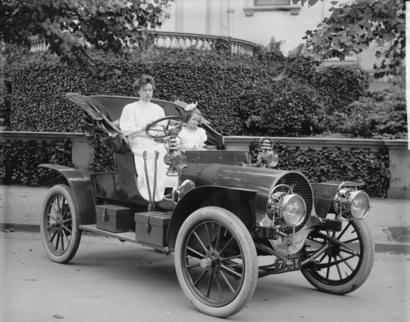
\includegraphics[width=\linewidth]{sample-franklin}
%   \caption{1907 Franklin Model D roadster. Photograph by Harris \&
%     Ewing, Inc. [Public domain], via Wikimedia
%     Commons. (\url{https://goo.gl/VLCRBB}).}
%   \Description{A woman and a girl in white dresses sit in an open car.}
% \end{figure}

% Your figures should contain a caption which describes the figure to
% the reader.

% Figure captions are placed {\itshape below} the figure.

% Every figure should also have a figure description unless it is purely
% decorative. These descriptions convey what’s in the image to someone
% who cannot see it. They are also used by search engine crawlers for
% indexing images, and when images cannot be loaded.

% A figure description must be unformatted plain text less than 2000
% characters long (including spaces).  {\bfseries Figure descriptions
%   should not repeat the figure caption – their purpose is to capture
%   important information that is not already provided in the caption or
%   the main text of the paper.} For figures that convey important and
% complex new information, a short text description may not be
% adequate. More complex alternative descriptions can be placed in an
% appendix and referenced in a short figure description. For example,
% provide a data table capturing the information in a bar chart, or a
% structured list representing a graph.  For additional information
% regarding how best to write figure descriptions and why doing this is
% so important, please see
% \url{https://www.acm.org/publications/taps/describing-figures/}.

% \subsection{The ``Teaser Figure''}

% A ``teaser figure'' is an image, or set of images in one figure, that
% are placed after all author and affiliation information, and before
% the body of the article, spanning the page. If you wish to have such a
% figure in your article, place the command immediately before the
% \verb|\maketitle| command:
% \begin{verbatim}
%   \begin{teaserfigure}
%     \includegraphics[width=\textwidth]{sampleteaser}
%     \caption{figure caption}
%     \Description{figure description}
%   \end{teaserfigure}
% \end{verbatim}

% \section{Citations and Bibliographies}

% The use of \BibTeX\ for the preparation and formatting of one's
% references is strongly recommended. Authors' names should be complete
% --- use full first names (``Donald E. Knuth'') not initials
% (``D. E. Knuth'') --- and the salient identifying features of a
% reference should be included: title, year, volume, number, pages,
% article DOI, etc.

% The bibliography is included in your source document with these two
% commands, placed just before the \verb|\end{document}| command:
% \begin{verbatim}
%   \bibliographystyle{ACM-Reference-Format}
%   \bibliography{bibfile}
% \end{verbatim}
% where ``\verb|bibfile|'' is the name, without the ``\verb|.bib|''
% suffix, of the \BibTeX\ file.

% Citations and references are numbered by default. A small number of
% ACM publications have citations and references formatted in the
% ``author year'' style; for these exceptions, please include this
% command in the {\bfseries preamble} (before the command
% ``\verb|\begin{document}|'') of your \LaTeX\ source:
% \begin{verbatim}
%   \citestyle{acmauthoryear}
% \end{verbatim}

%   Some examples.  A paginated journal article \cite{Abril07}, an
%   enumerated journal article \cite{Cohen07}, a reference to an entire
%   issue \cite{JCohen96}, a monograph (whole book) \cite{Kosiur01}, a
%   monograph/whole book in a series (see 2a in spec. document)
%   \cite{Harel79}, a divisible-book such as an anthology or compilation
%   \cite{Editor00} followed by the same example, however we only output
%   the series if the volume number is given \cite{Editor00a} (so
%   Editor00a's series should NOT be present since it has no vol. no.),
%   a chapter in a divisible book \cite{Spector90}, a chapter in a
%   divisible book in a series \cite{Douglass98}, a multi-volume work as
%   book \cite{Knuth97}, a couple of articles in a proceedings (of a
%   conference, symposium, workshop for example) (paginated proceedings
%   article) \cite{Andler79, Hagerup1993}, a proceedings article with
%   all possible elements \cite{Smith10}, an example of an enumerated
%   proceedings article \cite{VanGundy07}, an informally published work
%   \cite{Harel78}, a couple of preprints \cite{Bornmann2019,
%     AnzarootPBM14}, a doctoral dissertation \cite{Clarkson85}, a
%   master's thesis: \cite{anisi03}, an online document / world wide web
%   resource \cite{Thornburg01, Ablamowicz07, Poker06}, a video game
%   (Case 1) \cite{Obama08} and (Case 2) \cite{Novak03} and \cite{Lee05}
%   and (Case 3) a patent \cite{JoeScientist001}, work accepted for
%   publication \cite{rous08}, 'YYYYb'-test for prolific author
%   \cite{SaeediMEJ10} and \cite{SaeediJETC10}. Other cites might
%   contain 'duplicate' DOI and URLs (some SIAM articles)
%   \cite{Kirschmer:2010:AEI:1958016.1958018}. Boris / Barbara Beeton:
%   multi-volume works as books \cite{MR781536} and \cite{MR781537}. A
%   couple of citations with DOIs:
%   \cite{2004:ITE:1009386.1010128,Kirschmer:2010:AEI:1958016.1958018}. Online
%   citations: \cite{TUGInstmem, Thornburg01, CTANacmart}. Artifacts:
%   \cite{R} and \cite{UMassCitations}.

% \section{Acknowledgments}

% Identification of funding sources and other support, and thanks to
% individuals and groups that assisted in the research and the
% preparation of the work should be included in an acknowledgment
% section, which is placed just before the reference section in your
% document.

% This section has a special environment:
% \begin{verbatim}
%   \begin{acks}
%   ...
%   \end{acks}
% \end{verbatim}
% so that the information contained therein can be more easily collected
% during the article metadata extraction phase, and to ensure
% consistency in the spelling of the section heading.

% Authors should not prepare this section as a numbered or unnumbered {\verb|\section|}; please use the ``{\verb|acks|}'' environment.

% \section{Appendices}

% If your work needs an appendix, add it before the
% ``\verb|\end{document}|'' command at the conclusion of your source
% document.

% Start the appendix with the ``\verb|appendix|'' command:
% \begin{verbatim}
%   \appendix
% \end{verbatim}
% and note that in the appendix, sections are lettered, not
% numbered. This document has two appendices, demonstrating the section
% and subsection identification method.

% \section{Multi-language papers}

% Papers may be written in languages other than English or include
% titles, subtitles, keywords and abstracts in different languages (as a
% rule, a paper in a language other than English should include an
% English title and an English abstract).  Use \verb|language=...| for
% every language used in the paper.  The last language indicated is the
% main language of the paper.  For example, a French paper with
% additional titles and abstracts in English and German may start with
% the following command
% \begin{verbatim}
% \documentclass[sigconf, language=english, language=german,
%                language=french]{acmart}
% \end{verbatim}

% The title, subtitle, keywords and abstract will be typeset in the main
% language of the paper.  The commands \verb|\translatedXXX|, \verb|XXX|
% begin title, subtitle and keywords, can be used to set these elements
% in the other languages.  The environment \verb|translatedabstract| is
% used to set the translation of the abstract.  These commands and
% environment have a mandatory first argument: the language of the
% second argument.  See \verb|sample-sigconf-i13n.tex| file for examples
% of their usage.

% \section{SIGCHI Extended Abstracts}

% The ``\verb|sigchi-a|'' template style (available only in \LaTeX\ and
% not in Word) produces a landscape-orientation formatted article, with
% a wide left margin. Three environments are available for use with the
% ``\verb|sigchi-a|'' template style, and produce formatted output in
% the margin:
% \begin{itemize}
% \item {\verb|sidebar|}:  Place formatted text in the margin.
% \item {\verb|marginfigure|}: Place a figure in the margin.
% \item {\verb|margintable|}: Place a table in the margin.
% \end{itemize}

% %%
% %% The acknowledgments section is defined using the "acks" environment
% %% (and NOT an unnumbered section). This ensures the proper
% %% identification of the section in the article metadata, and the
% %% consistent spelling of the heading.
% \begin{acks}
% To Robert, for the bagels and explaining CMYK and color spaces.
% \end{acks}

% %%
% %% The next two lines define the bibliography style to be used, and
% %% the bibliography file.
% \bibliographystyle{ACM-Reference-Format}
% \bibliography{sample-base}

% %%
% %% If your work has an appendix, this is the place to put it.
% \appendix

% \section{Research Methods}

% \subsection{Part One}

% Lorem ipsum dolor sit amet, consectetur adipiscing elit. Morbi
% malesuada, quam in pulvinar varius, metus nunc fermentum urna, id
% sollicitudin purus odio sit amet enim. Aliquam ullamcorper eu ipsum
% vel mollis. Curabitur quis dictum nisl. Phasellus vel semper risus, et
% lacinia dolor. Integer ultricies commodo sem nec semper.

% \subsection{Part Two}

% Etiam commodo feugiat nisl pulvinar pellentesque. Etiam auctor sodales
% ligula, non varius nibh pulvinar semper. Suspendisse nec lectus non
% ipsum convallis congue hendrerit vitae sapien. Donec at laoreet
% eros. Vivamus non purus placerat, scelerisque diam eu, cursus
% ante. Etiam aliquam tortor auctor efficitur mattis.

% \section{Online Resources}

% Nam id fermentum dui. Suspendisse sagittis tortor a nulla mollis, in
% pulvinar ex pretium. Sed interdum orci quis metus euismod, et sagittis
% enim maximus. Vestibulum gravida massa ut felis suscipit
% congue. Quisque mattis elit a risus ultrices commodo venenatis eget
% dui. Etiam sagittis eleifend elementum.

% Nam interdum magna at lectus dignissim, ac dignissim lorem
% rhoncus. Maecenas eu arcu ac neque placerat aliquam. Nunc pulvinar
% massa et mattis lacinia.

\end{document}
\endinput
%%
%% End of file `sample-manuscript.tex'.
